\documentclass[a4paper, 12pt]{article}
\usepackage[utf8]{inputenc}
\usepackage[czech]{babel}
\usepackage[left=2cm, top=3cm, text={17cm, 24cm}]{geometry}
\usepackage{graphicx}
\usepackage{fancyhdr}
\usepackage{enumitem}
\usepackage[T1]{fontenc}
\usepackage{tikz}
\usepackage{tikz-qtree}
\usetikzlibrary{shapes.geometric}
\usetikzlibrary{calc,shapes.multipart,chains,arrows}
\makeatletter
\newcommand*{\rom}[1]{\expandafter\@slowromancap\romannumeral #1@}
\makeatother
\usepackage[unicode]{hyperref}
\hypersetup{
	colorlinks = true,
	hypertexnames = true,
	citecolor = red
}

\setlength{\headheight}{15pt}

% TODO
% - popisky obrazku

%\title{ifj_dokumentace}
%\author{xchoch09 }
%\date{December 2021}

\begin{document}

    %Titulni strana
    \begin{titlepage}
        \begin{center}
            
\includegraphics[width=0.87\textwidth]{images/logo_cz.png}
            \vspace*{6cm}

            \Huge{\textbf{Dokumentace}}
            \vspace{0.5cm}
            
            \LARGE{Implementace překladače imperativního jazyka IFJ21}
            \vspace{0.5cm}
            
            \Large{Tým 035, varianta \rom{1}}
            \vspace{2.5cm}
            
            \large{\textbf{vedoucí} Štěpán Bakaj (xbakaj00) 25\%}
            \vspace{0.1cm}
            
            \large{David Chocholatý (xchoch09) 25\%}
            \vspace{0.1cm}
            
            \large{Adam Kaňkovský (xkanko00) 25\%}
            \vspace{0.1cm}
            
            \large{Radek Šerejch (xserej00) 25\%}
            \vspace{0.1cm}
            
           \vfill
		   \begin{flushleft} 
		   \large
		   Bez implementace rozšíření
		   \hfill
		   Brno, \today
		   \end{flushleft}
        \end{center}
    \end{titlepage}

\pagestyle{fancy}
\lhead{\bfseries Dokumentace}
\rhead{\bfseries Obsah}

\newpage
\tableofcontents
\newpage

\rhead{\bfseries Práce v týmu}
\section{Práce v týmu}
\subsection{Rozdělení práce mezi jednotlivé členy týmu}
\begin{itemize}
    \begin{minipage}{0.25\linewidth}   
        \item Štěpán Bakaj
        \item[]\item[]\item[]\item[]\item[]\item[]\item[]
        \item David Chocholatý
        \item[]\item[]\item[]\item[]\item[]\item[]\item[]
        \item Adam Kaňkovský
        \item[]\item[]\item[]\item[]\item[]\item[]\item[]
        \item Radek Šerejch
        \item[]\item[]\item[]\item[]\item[]\item[]\item[]
        \vspace{0.25cm}
    \end{minipage}
    \begin{minipage}{0.7\linewidth}
        \item[-] návrh automatu pro lexikální analýzu
        \item[-] datový typ string\_t a zásobník symbolů
        \item[-] obousměrně vázaný seznam (dll)
        \item[-] návrh precedenční tabulky
        \item[-] implementace syntaktického analyzátoru (psa)
        \item[-] implementace sémantického analyzátoru (psa)
        \item[-] testování, překlad a spuštění překladače
        \item[]
        
        \item[-] návrh automatu pro lexikální analýzu
        \item[-] implementace lexikálního analyzátoru
        \item[-] zásobník parametrů a jednosměrně vázaný seznam (ids\_list\_t)
        \item[-] LL gramatika a LL tabulka
        \item[-] implementace syntaktického analyzátoru (parser)
        \item[-] implementace sémantického analyzátoru (parser)
        \item[-] testování a dokumentace
        \item[]
        
        \item[-] návrh automatu pro lexikální analýzu
        \item[-] datové typy pro lexikální analyzátor
        \item[-] návrh precedenční tabulky a tabulky symbolů
        \item[-] binární vyhledávací strom
        \item[-] jednosměrně vázaný seznam (sym\_linked\_list)
        \item[-] generování kódu
        \item[-] testování (sémantický analyzátor, generování kódu)
        \item[]
        
        \item[-] návrh automatu pro lexikální analýzu
        \item[-] datový typ token\_t
        \item[-] implementace lexikálního analyzátoru
        \item[-] návrh precedenční tabulky
        \item[-] implementace syntaktického analyzátoru (psa)
        \item[-] implementace sémantického analyzátoru (psa)
        \item[-] testování (lexikální analyzátor, syntaktický analyzátor)
        \item[-] generování kódu (psa)
    \end{minipage}
\end{itemize}

\newpage

\rhead{\bfseries Implementace překladače (Lexikální analýza)}
\section{Implementace překladače}
\subsection{Lexikální analýza}
\subsubsection{Základní struktura lexikálního analyzátoru}
Lexikální analyzátor je implementován v souboru \textit{scanner.c (.h)}. Jeho hlavní funkcí implementující vnitřní logiku je funkce \textit{\textbf{get\_next\_token()}}. Načítání znaků ze standardního vstupu \textit{stdin} probíhá pomocí cyklu \textit{while}. Znaky jsou načítány, dokud není na vstupu konec souboru \textit{EOF}. Pokaždé, kdy konečný automat přejde do koncového stavu je provádění funkce ukončeno a je navrácen načtený token. Při opětovném zavolání funkce je v cyklu \textit{while} čten opět následující znak ze vstupu. Po ukončení provádění výše zmíněného cyklu bez stavu, který by navracel token, a tím ukončil provádění funkce, je kontrolováno, zda se konečný automat nachází v koncovém stavu. Tato situace je validní, pokud se konečný automat nachází v počátečním a zároveň koncovém stavu \textit{init}. Funkce \textit{get\_next\_token()} navrací hodnotu datového typu \textit{token\_t*}, který obsahuje typ tokenu a jeho atribut. Datový typ atributu je odvozen na základě typu tokenu. Definice datového typu \textit{token\_t} je implementována v souboru \textit{scanner.h}.

\subsubsection{Rozhraní pro syntaktický analyzátor}
Rozhraní mezi lexikálním (\textit{scanner}) a syntaktickým (\textit{parser, psa}) analyzátorem tvoří dvě funkce. První z nich je funkce \textit{\textbf{get\_next\_token()}}, načítající vstupní tokeny, a druhá je funkce \newline \textit{\textbf{delete\_token()}}, která slouží pro uvolnění paměti zaalokované pro již načtený token.

\vspace{4cm}

\begin{figure}[ht!]
\begin{center}
    \begin{tikzpicture}[square/.style={regular polygon,regular polygon sides=4}]
            \node at (0,0) [square, draw] {SCANNER};
            \node at (12,0) [square, draw] {PARSER, PSA};
            \draw (1.65,1) -- node[above]{get\_next\_token()} (9.85,1);
            \draw (1.65,-1) -- node[above]{delete\_token()} (9.85,-1);
    \end{tikzpicture}
\caption{Rozhraní mezi lexikálním a syntaktickým analyzátorem}
\end{center}
\end{figure}

\newpage

\subsubsection{Diagram konečného automatu}
\begin{figure}[ht!]
\begin{center}
  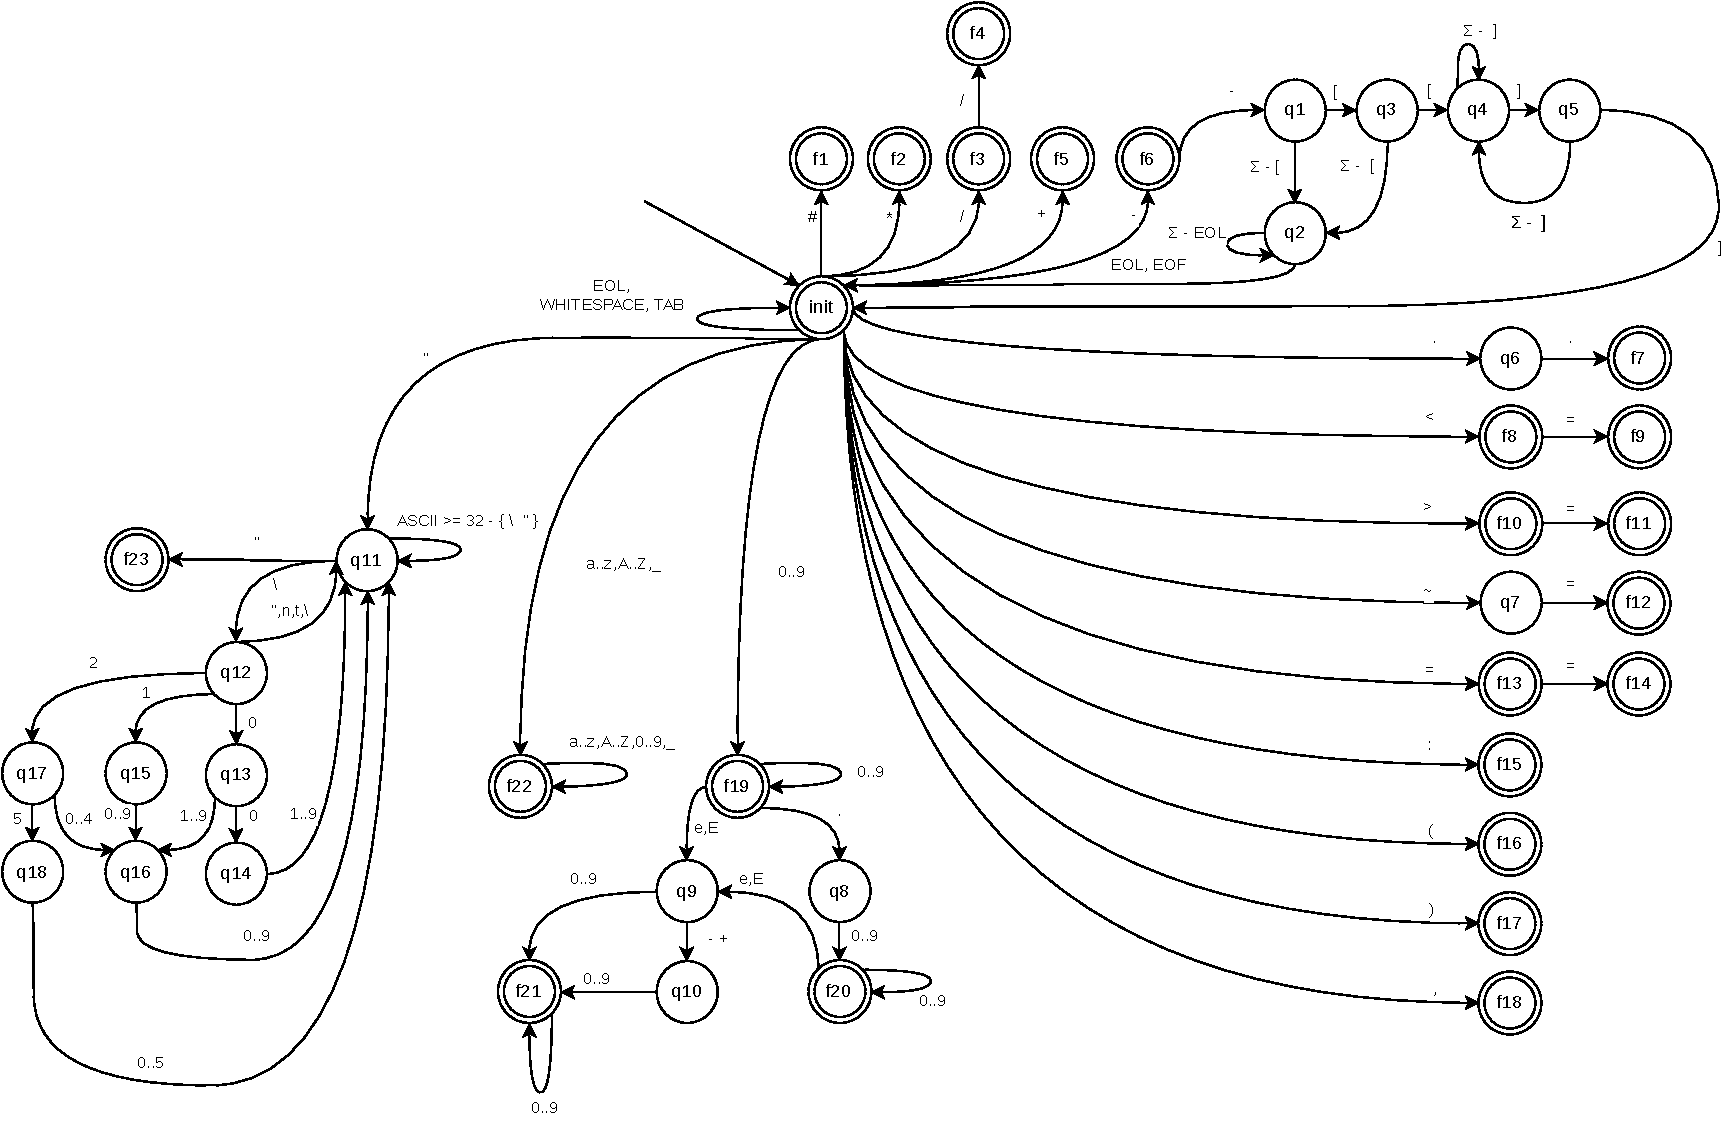
\includegraphics[angle=90,origin=c, width=0.8\textwidth]{images/IFJ2021_FSM_final.pdf}
  \caption{Diagram konečného automatu}
\end{center}
\end{figure}

\subsubsection{Legenda diagramu konečného automatu}

\begin{itemize}
    \begin{minipage}{0.05\linewidth}   
        \item \textbf{q1}
        \item \textbf{q2}
        \item \textbf{q3}
        \item \textbf{q4}
        \item \textbf{q5}
        \item \textbf{q6}
        \item \textbf{q7}
        \item \textbf{q8}
        \item \textbf{q9}
        \vspace{4cm}
        \item \textbf{f1}
        \item \textbf{f2}
        \item \textbf{f3}
        \item \textbf{f4}
        \item \textbf{f5}
        \item \textbf{f6}
        \item \textbf{f7}
        \item \textbf{f8}
        \item \textbf{f9}
        \item \textbf{f10}
        \item \textbf{f11}
        
    \end{minipage}
    \begin{minipage}{0.55\linewidth}
        \item[] S\_ONE\_LINE\_COMMENT
        \item[] S\_ONE\_LINE\_COMMENT\_CONTENT
        \item[] S\_LEFT\_SQUARE\_BRACKET
        \item[] S\_BLOCK\_COMMENT\_CONTENT
        \item[] S\_RIGHT\_SQUARE\_BRACKET
        \item[] S\_DOT
        \item[] S\_TILDE
        \item[] S\_DECIMAL\_POINT
        \item[] S\_EXP
        \vspace{4cm}
        \item[] S\_CHAR\_CNT
        \item[] S\_MUL
        \item[] S\_DIV
        \item[] S\_INT\_DIV
        \item[] S\_PLUS
        \item[] S\_MINUS
        \item[] S\_CONCAT
        \item[] S\_LESS\_THAN
        \item[] S\_LESS\_EQ
        \item[] S\_GTR\_THAN
        \item[] S\_GTR\_EQ
        
    \end{minipage}
    \begin{minipage}{0.06\linewidth}
        \vspace{0.55cm}
        \item \textbf{q10}
        \item \textbf{q11}
        \item \textbf{q12}
        \item \textbf{q13}
        \item \textbf{q14}
        \item \textbf{q15}
        \item \textbf{q16}
        \item \textbf{q17}
        \item \textbf{q18}
        \vspace{4cm}
        \item \textbf{f12}
        \item \textbf{f13}
        \item \textbf{f14}
        \item \textbf{f15}
        \item \textbf{f16}
        \item \textbf{f17}
        \item \textbf{f18}
        \item \textbf{f19}
        \item \textbf{f20}
        \item \textbf{f21}
        \item \textbf{f22}
        \item \textbf{f23}
        
    \end{minipage}
    \begin{minipage}{0.4\linewidth}
        \vspace{0.55cm}
        \item[] S\_EXP\_PLUS\_MINUS
        \item[] S\_STRING\_CONTENT
        \item[] S\_ESC\_SEQ\_BACKSLASH
        \item[] S\_ESC\_SEQ\_ZERO
        \item[] S\_ESC\_SEQ\_DOUBLE\_ZERO
        \item[] S\_ESC\_SEQ\_ONE
        \item[] S\_ESC\_SEQ\_X\_X
        \item[] S\_ESC\_SEQ\_TWO
        \item[] S\_ESC\_SEQ\_TWO\_FIVE
        \vspace{4cm}
        \item[] S\_NOT\_EQ
        \item[] S\_ASSIGN
        \item[] S\_EQ
        \item[] S\_COLON
        \item[] S\_LEFT\_BRACKET
        \item[] S\_RIGHT\_BRACKET
        \item[] S\_COMMA
        \item[] S\_INT
        \item[] S\_DECIMAL
        \item[] S\_DECIMAL\_W\_EXP
        \item[] S\_IDENTIFIER\_KEYWORD
        \item[] S\_STRING
    \end{minipage}
\end{itemize}

\newpage

\rhead{\bfseries Implementace překladače (Syntaktická analýza)}
\subsection{Syntaktická analýza}
\subsubsection{Parser}
Implementace parseru se nachází v souboru \textit{parser.c (.h)}. Syntaktická část parseru implementuje syntaktickou analýzu založenou na LL gramatice metodou rekurzivního sestupu \cite{FITPUB8538}. Výše zmíněný soubor obsahuje také z pohledu logiky hlavní funkci celého překladače: \textit{\textbf{parser()}}. Tato funkce provádí všechny nezbytné úkony před započetím analýzy i po jejím skončení a volá funkci \textit{prog()}, která zpracovává počáteční pravidlo (prolog) každého vstupního programu. Všechny potřebné parametry pro zpracování syntaktické a sémantické analýzy vstupního programu jsou uloženy ve struktuře, která je předávána jako parametr pomocí ukazatele. Tento parametr je datového typu \textit{p\_data\_ptr\_t}. Načtení tokenu lexikálním analyzátorem se provádí pomocí funkce \textit{\textbf{next\_token()}}. Ta zajišťuje zavolání obou funkcí sloužících jako rozhraní mezi lexikálním a syntaktickým analyzátorem, a to funkcí \textit{delete\_token()} pro uvolnění paměti již zpracovaného tokenu a \textit{get\_next\_token()} pro načtení následujícího tokenu. Parser zpracovává všechny části LL gramatiky až na výrazy. Ty jsou předávány pro zpracování metodou precedenční syntaktické analýzy.

\subsubsection{Rozhraní mezi parserem a zpracováním výrazů (psa)}
Rozhraní mezi parserem a zpracováním výrazů (psa) tvoří funkce \textit{\textbf{psa()}}. Ta je v parseru zapouzdřena do funkce \textit{expression()}. Jako parametr funkce \textit{psa()} je opět předáván ukazatel na strukturu obsahující všechna potřebná data datového typu p\_data\_ptr\_t. Část syntaktického analyzátoru pro zpracování výrazů využívá funkci \textit{next\_token()} pro zpracování vstupních tokenů.

\vspace{4cm}

\begin{figure}[ht!]
\begin{center}
\begin{tikzpicture}[square/.style={regular polygon,regular polygon sides=4}]
        \node at (0,0) [square, draw] {PARSER};
        \node at (12,0) [square, draw] {Zpracování výrazů};
        \draw (1.4,1) -- node[above]{psa()} (9.45,1);
        \draw (1.4,-1) -- node[above]{next\_token()} (9.45,-1);
\end{tikzpicture}
\caption{Rozhraní mezi parserem a zpracováním výrazů}
\end{center}
\end{figure}

\newpage

\subsubsection{LL gramatika}

\begin{enumerate}
    \item <prog> → require “ifj21” <main\_b>
    \item[]
    \item <main\_b> → function id (<params>) <ret\_func\_types> <stats> end <main\_b>
    \item <main\_b> → global id : function (<arg\_def\_types>) <ret\_def\_types> <main\_b>
    \item <main\_b> → id (<args>) <main\_b>
    \item <main\_b> → $\varepsilon$
    \item[]
    \item <stats> → local id : <type> <assign> <stats>
    \item <stats> → if exp then <stats> else <stats> end <stats>
    \item <stats> → while exp do <stats> end <stats>
    \item <stats> → return <ret\_vals> <stats>
    \item <stats> → id <id\_func> <stats>
    \item <stats> → $\varepsilon$
    \item[]
    \item <id\_func> → <n\_ids> = <as\_vals>
    \item <id\_func> → (<args>)
    \item[]
    \item <params> → id : <type> <n\_params>
    \item <params> → $\varepsilon$
    \item <n\_params> → , id : <type> <n\_params>
    \item <n\_params> → $\varepsilon$
    \item[]
    \item <n\_ids> → , id <n\_ids>
    \item <n\_ids> → $\varepsilon$
    \item[]
    \item <vals> → exp <n\_vals>
    \item <n\_vals> → , exp <n\_vals>
    \item <n\_vals> → $\varepsilon$
    \item[]
    \item <as\_vals> → <vals>
    \item <as\_vals> → id (<args>)
    \item[]
    \item <ret\_vals> → <vals>
    \item <ret\_vals> → $\varepsilon$
    \item[]
    \item <assign> → = <assign\_val>
    \item <assign> → $\varepsilon$
    \item[]
    \item <assign\_val> → exp
    \item <assign\_val> → id (<args>)
    \item[]
    \item <term> → id
    \item <term> → <const>
    \item[]
    \item <args> → <term> <n\_args>
    \item[]
    \item <args> → $\varepsilon$
    \item <n\_args> → , <term> <n\_args>
    \item <n\_args> → $\varepsilon$
    \item[]
    \item <arg\_def\_types> → <func\_def\_types>
    \item <arg\_def\_types> → $\varepsilon$
    \item[]
    \item <ret\_func\_types> → : <func\_types>
    \item <ret\_func\_types> → $\varepsilon$
    \item[]
    \item <ret\_def\_types> → : <func\_def\_types>
    \item <ret\_def\_types> → $\varepsilon$
    \item[]
    \item <func\_types> → <type>  <n\_func\_types>
    \item <n\_func\_types> → , <type>  <n\_func\_types>
    \item <n\_func\_types> → $\varepsilon$
    \item[]
    \item <func\_def\_types> → <type>  <n\_func\_def\_types>
    \item <n\_func\_def\_types> → , <type>  <n\_func\_def\_types>
    \item <n\_func\_def\_types> → $\varepsilon$
    \item[]
    \item <type> → integer
    \item <type> → number
    \item <type> → string
    \item <type> → nil
    \item[]
    \item <const> → int\_value
    \item <const> → double\_value
    \item <const> → string\_value
    \item <const> → nil
\end{enumerate}

\vspace{1cm}
Poznámka: "exp" - označení pro výraz

\newpage

\subsubsection{LL tabulka}
\begin{figure}[ht!]
\begin{center}
  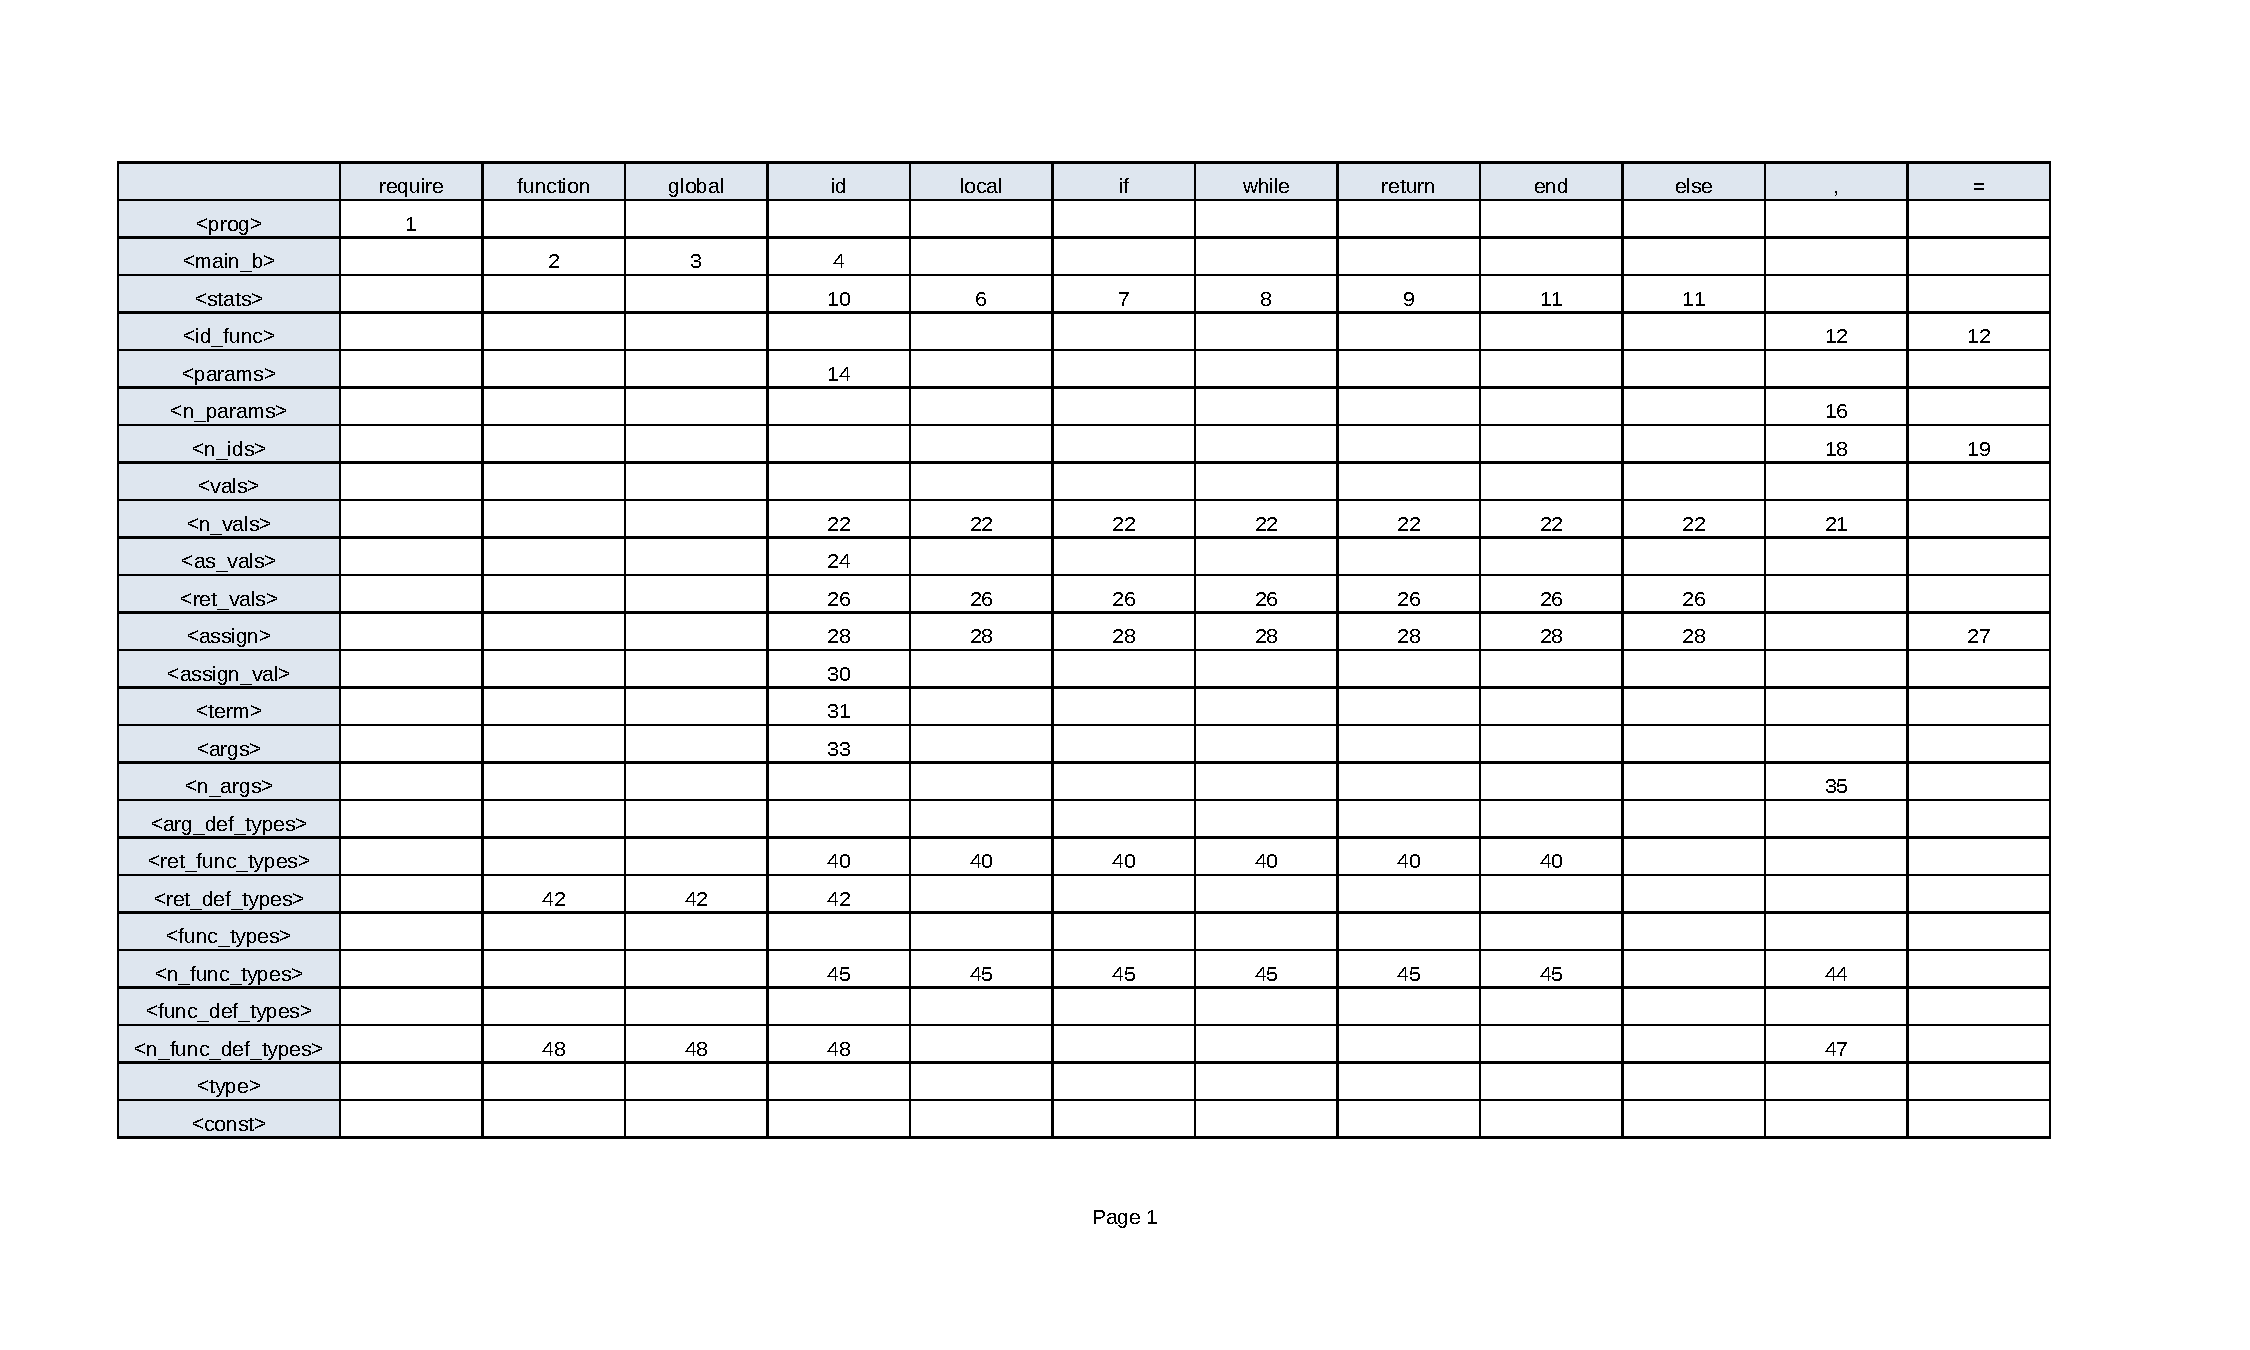
\includegraphics[angle=90,origin=c, width=0.59\textwidth, trim={0 2.5cm 0 2.5cm},clip]{images/LL_table_1.pdf}
  \caption{LL tabulka, část 1}
\end{center}
\end{figure}


\newpage

\begin{figure}[ht!]
\begin{center}
  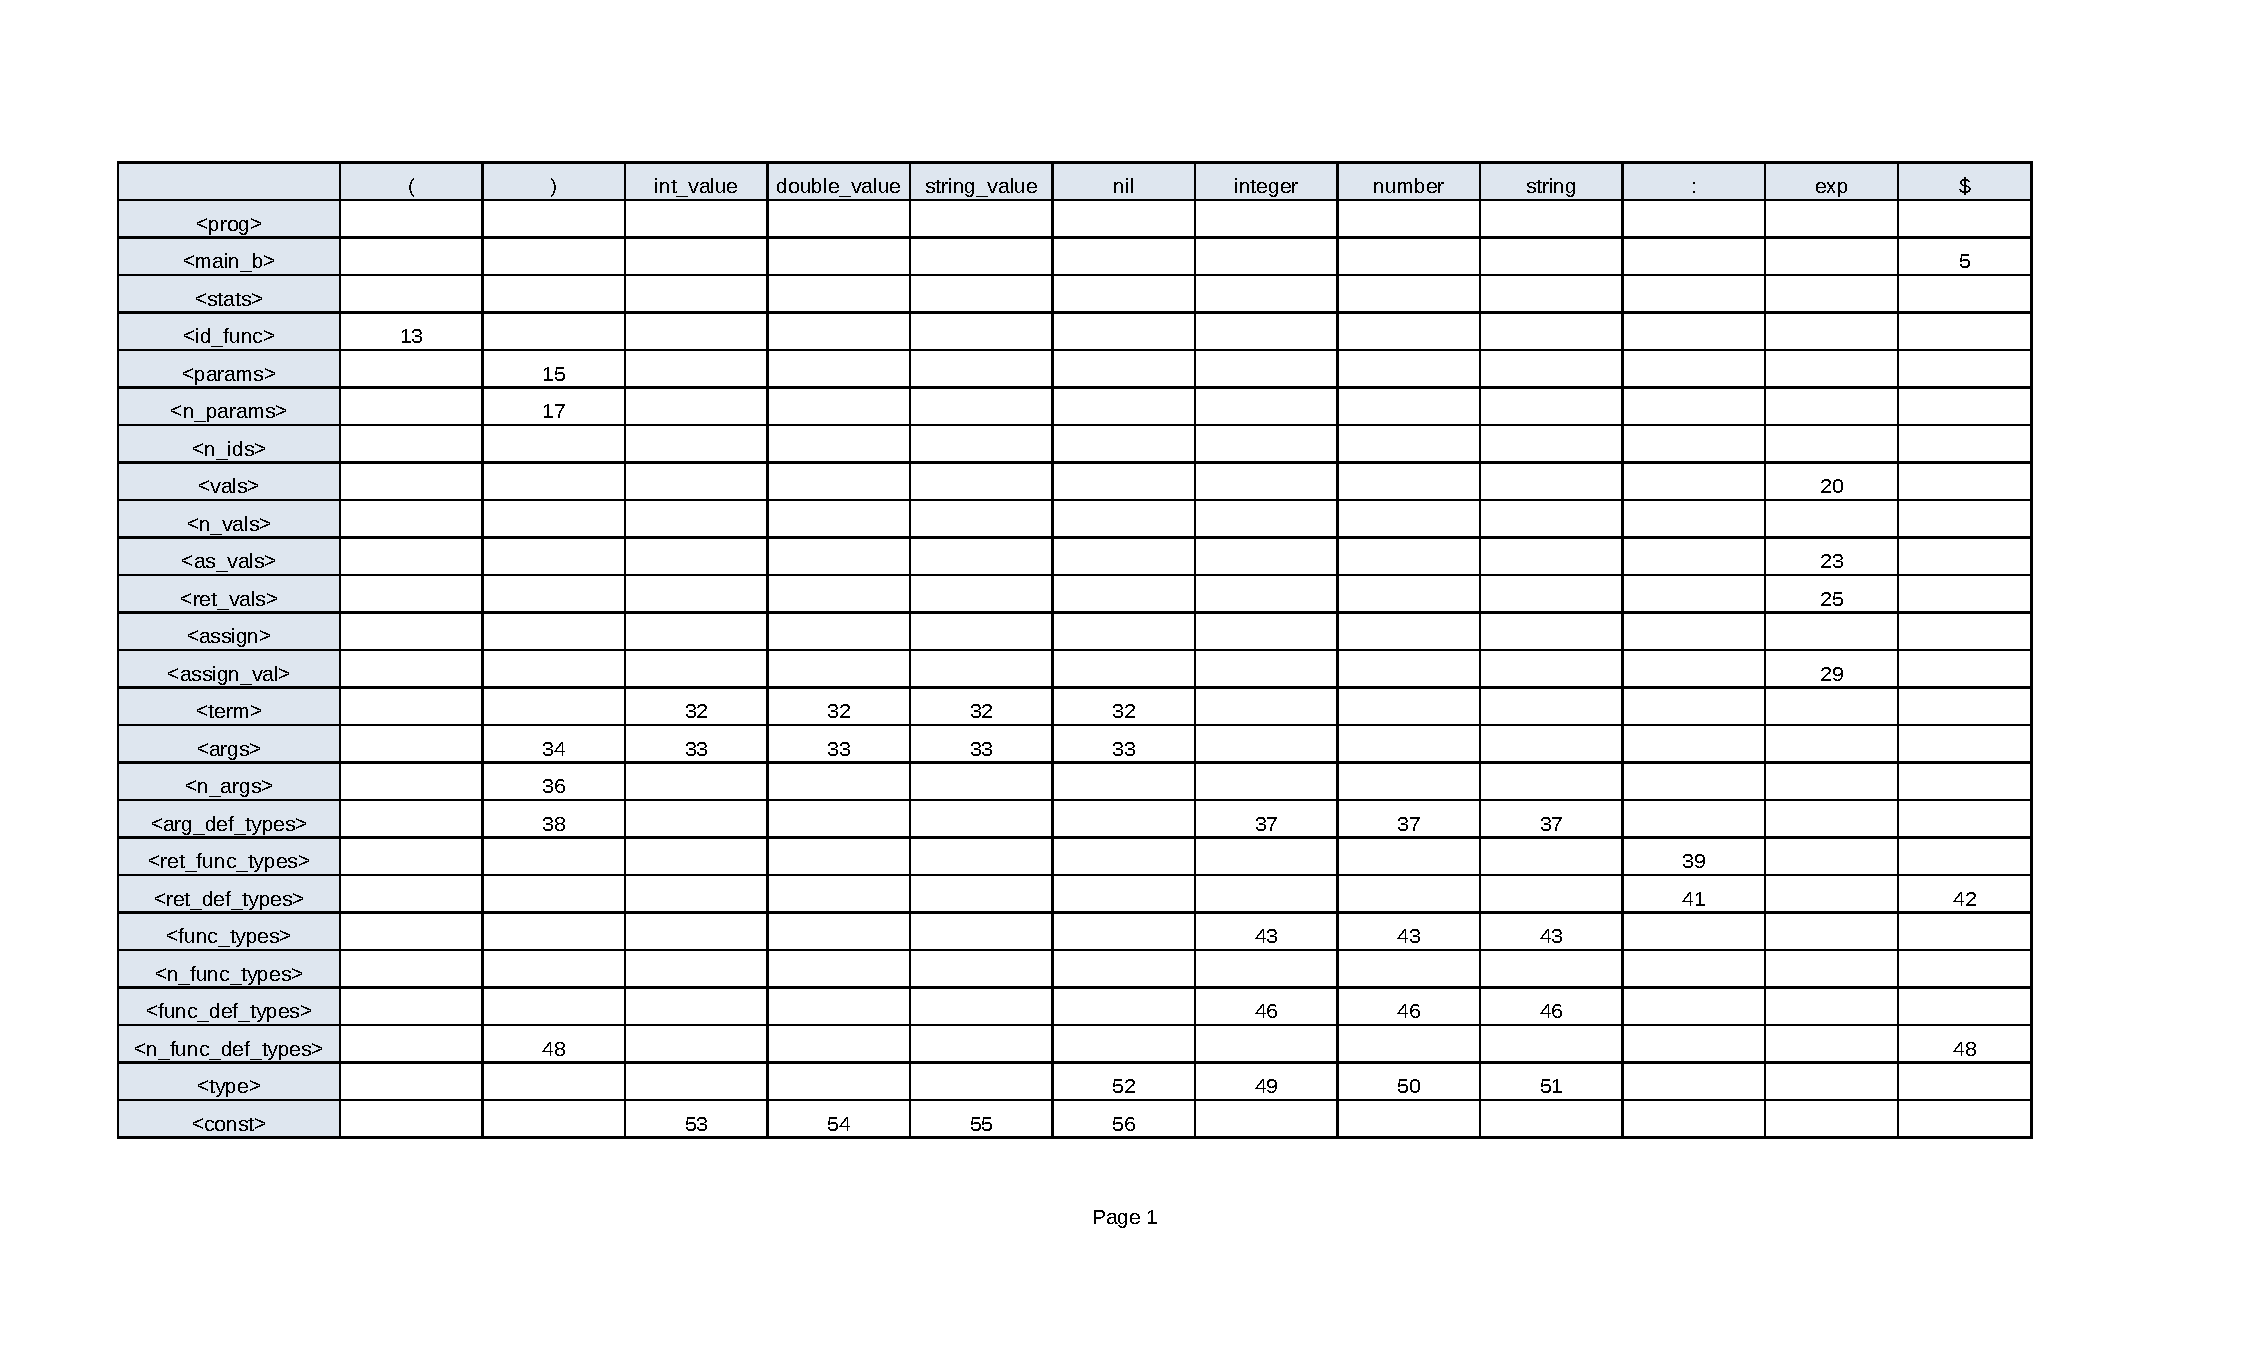
\includegraphics[angle=90,origin=c, width=0.59\textwidth, trim={0 2.5cm 0 2.5cm},clip]{images/LL_table_2.pdf}
  \caption{LL tabulka, část 2}
\end{center}
\end{figure}

\newpage

\subsubsection{Zpracování výrazů}
Zpracování výrazů je implementováno v souboru \textit{psa.c (.h)}. To je prováděno metodou precedenční syntaktické analýzy \cite{FITPUB8538}. Nejprve je nainicializován zásobník (kapitola 3.1.1), kam se postupně budou ukládat symboly z precedenční tabulky, a na vrchol je vložen znak reprezentující konec čtení. Symboly jsou datového typu \textit{psa\_table\_symbol\_enum}. Poté je načten symbol z vrcholu zásobníku a symbol ze vstupu. Pro tyto symboly jsou určeny indexy pro čtení z precedenční tabulky (funkce \textit{\textbf{get\_index\_enum()}} a \textit{\textbf{get\_index\_ token()}}). Podle vyčtené hodnoty je buď přidán symbol na zásobník bez zarážky, se zarážkou, anebo je spuštěna redukce části výrazu na zásobníku. Redukce výrazu se provádí tím způsobem, že je nejprve určeno, kolik symbolů se nachází na vrcholu zásobníku do zarážky. Maximálně se může jednat o tři symboly. Poté pomocí funkce \textit{\textbf{test\_rule()}} se zjistí, zda existuje pro dané symboly pravidlo na redukci. Pravidla jsou definována v \textit{psa\_rules\_enum}. Pomocí daného pravidla se zredukuje část výrazu. Redukce výrazu proběhne úspěšně pouze tehdy, pokud je na vstupu token daného výrazu a na vrcholu zásobníku je symbol pro konec čtení (počítáno bez výsledného neterminálu).

\subsubsection{Precedenční tabulka}
\begin{figure}[ht!]
\begin{center}
  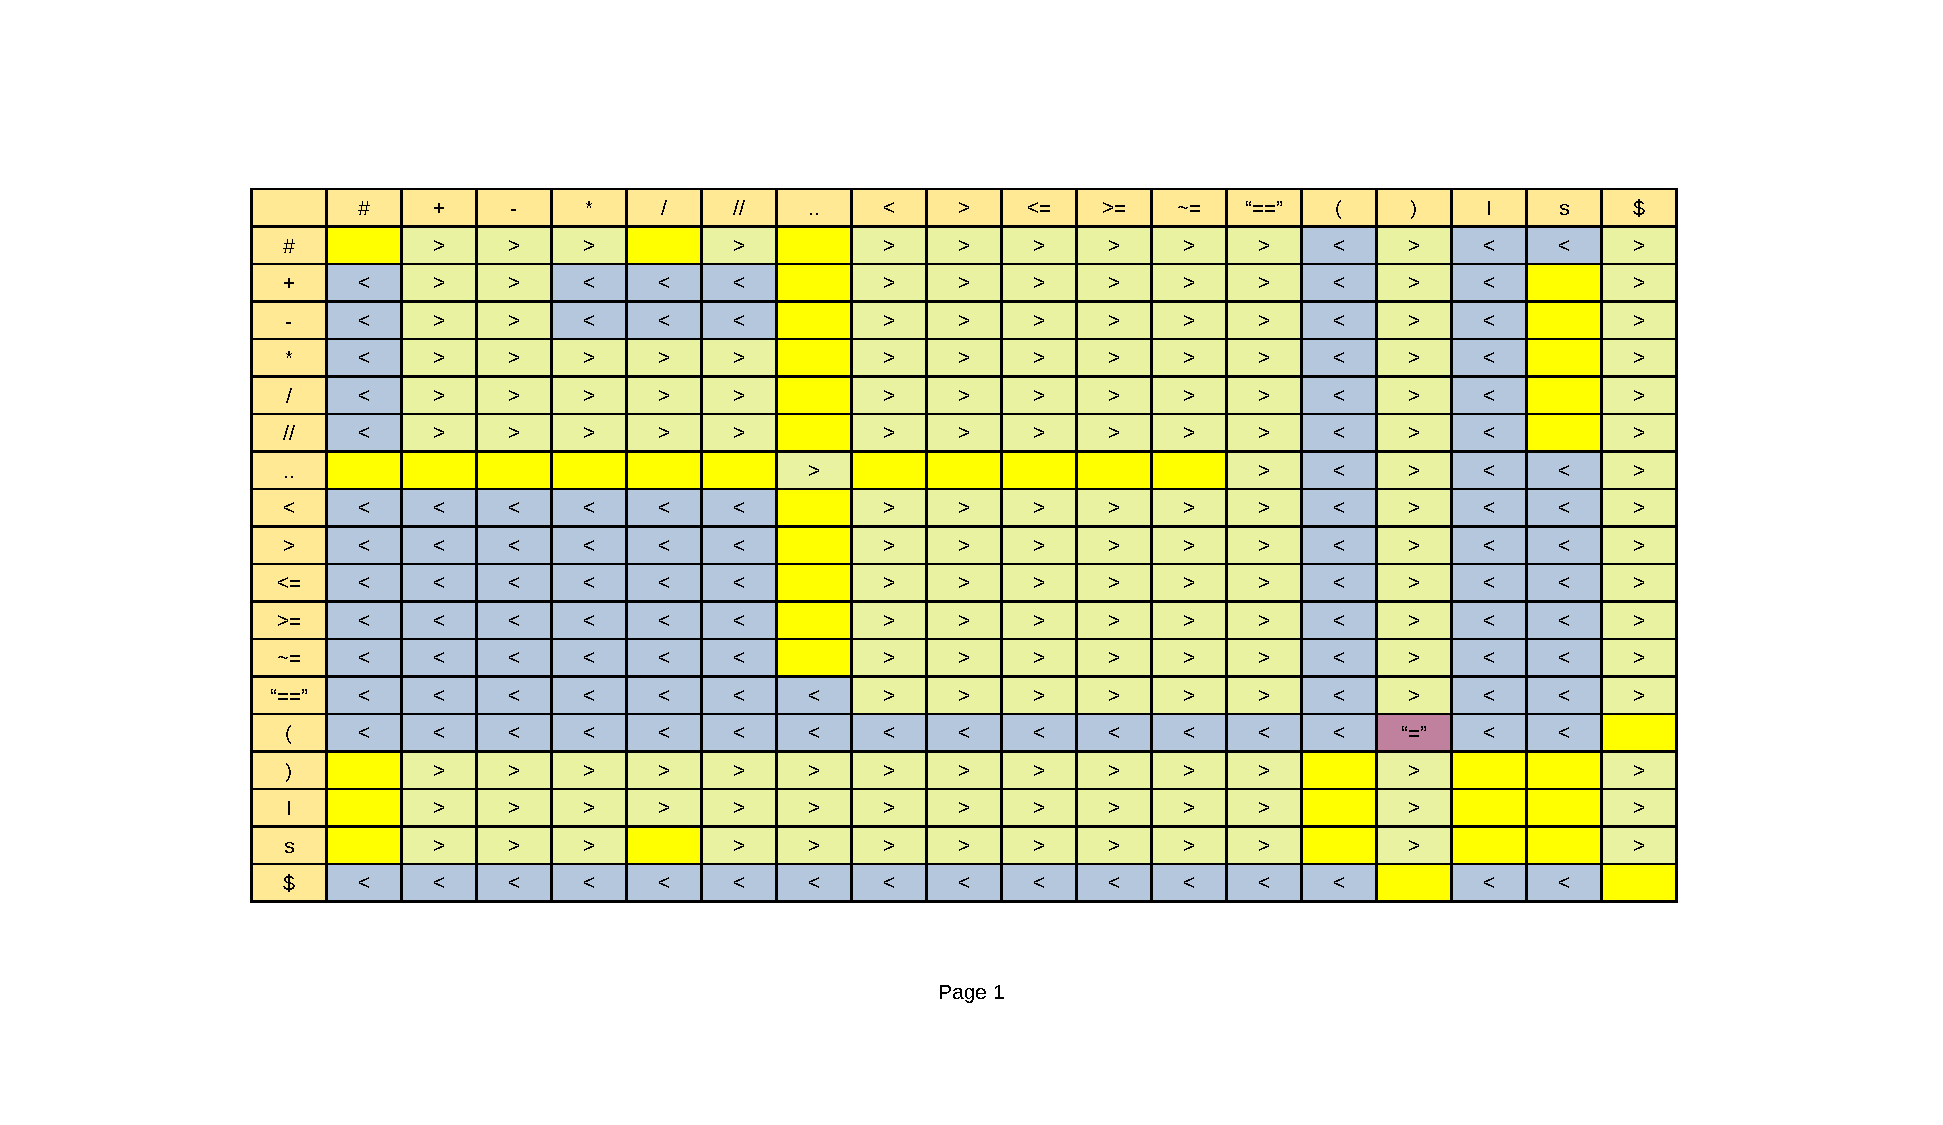
\includegraphics[width=1\textwidth, trim={0 2.5cm 0 0},clip]{images/precedence_table.pdf}
  \caption{Precedenční tabulka}
\end{center}
\end{figure}

\newpage

\subsubsection{Gramatika pro výrazy}

\begin{enumerate}
    \item E → i
    \item E → $\#$E
    \item E → (E)
    \item E → E $..$ E
    \item E → E $+$ E
    \item E → E $-$ E
    \item E → E $*$ E
    \item E → E $/$ E
    \item E → E $//$ E
    \item E → E $=$ E
    \item E → E $\sim=$ E
    \item E → E $<=$ E
    \item E → E $>=$ E
    \item E → E $<$ E
    \item E → E $>$ E
\end{enumerate}

\newpage

\rhead{\bfseries Implementace překladače (Tabulka symbolů)}
\subsection{Tabulka symbolů}
Dle výběru varianty zadání \rom{1} je tabulka symbolů implementována binárním vyhledávacím stromem. Ten je implementován v souboru \textit{symtable.c (.h)}.

\subsubsection{Návrh tabulky symbolů}
Prvek v tabulce symbolů obsahuje následující elementy:

\vspace{1cm}

\begin{itemize}
    \begin{minipage}{0.3\linewidth}   
    \item declared
    \item defined
    \item data\_type
    \item params\_count
    \item params\_type\_count
    \item returns\_def\_count
    \item returns\_count    
    \item first\_param
    \item first\_type\_param
    \item first\_def\_ret
    \item first\_ret
    \end{minipage}
    \begin{minipage}{0.65\linewidth}   
    \item[-] proměnná/funkce byla deklarována
    \item[-] proměnná/funkce byla definována
    \item[-] datový typ proměnné
    \item[-] počet parametrů definice funkce
    \item[-] počet parametrů deklarace funkce
    \item[-] počet návratových typů definice funkce
    \item[-] počet návratových typů deklarace funkce    
    \item[-] ukazatel na první parametr definice funkce
    \item[-] ukazatel na první parametr deklarace funkce
    \item[-] ukazatel na první návratový typ definice funkce
    \item[-] ukazatel na první návratový typ deklarace funkce
    \end{minipage}
\end{itemize}

\vspace{1cm}

Všechny elementy prvku v tabulce jsou uloženy ve struktuře datového typu \textit{symData\_t}. Při inicializaci dat prvku jsou všechny elementy nastaveny na výchozí hodnotu a prvek pracuje pouze s ukazatelem na danou strukturu.

Jako element prvku tabulky symbolů není ukládána informace, zda daný identifikátor patří proměnné nebo funkci. Tuto informaci lze vydedukovat z definice jazyka. Pokud-li se nachází identifikátor v tabulce jiné než globální (tedy v lokální tabulce), jedná se o identifikátor proměnné (v jazyku IFJ21 nelze definovat vnořené funkce a v hlavním těle programu nelze deklarovat proměnné). Naopak jestliže se identifikátor nachází v globální tabulce, jedná se o identifikátor funkce.

\newpage

\subsubsection{Uložení tabulek symbolů do jednosměrně vázaného seznamu}
Jednotlivé tabulky symbolů jsou vloženy do jednosměrně vázaného seznamu. Jeho implementace se nachází v souboru \textit{sym\_linked\_list.c (.h)}. Tento způsob uložení tabulky reprezentující blok slouží pro vyhledávání identifikátoru proměnné v tabulkách symbolů. Lineární procházení seznamu se využívá při ověřování deklarace či definice proměnné. Identifikátory funkcí se nachází pouze v úplně posledním prvku seznamu a to v tabulce reprezentující globální tabulku celého programu.

\vspace{4cm}

\begin{figure}[ht!]
\begin{center}
\begin{tikzpicture}[list/.style={rectangle split, rectangle split parts=2,
    draw, rectangle split horizontal}, >=stealth, start chain]

  \node[list,on chain] (A) {lok. tab. symb. *};
  \node[list,on chain] (B) {lok. tab. symb. *};
  \node[list,on chain] (C) {glob. tab. symb. *};
  \node[on chain,draw,inner sep=6pt] (D) {};
  \draw (D.north east) -- (D.south west);
  \draw (D.north west) -- (D.south east);
  \draw[*->] let \p1 = (A.two), \p2 = (A.center) in (\x1,\y2) -- (B);
  \draw[*->] let \p1 = (B.two), \p2 = (B.center) in (\x1,\y2) -- (C);
  \draw[*->] let \p1 = (C.two), \p2 = (C.center) in (\x1,\y2) -- (D);
\end{tikzpicture}

\tikzset{every tree node/.style={minimum width=2em,draw,circle},
         blank/.style={draw=none},
         edge from parent/.style=
         {draw,edge from parent path={(\tikzparentnode) -- (\tikzchildnode)}},
         level distance=1.5cm}
\begin{tikzpicture}[sibling distance=25pt]
\Tree
[.ida     
    [.idb ]
    [.idc 
    \edge[blank]; \node[blank]{};
    \edge[]; [.idd
         ]
    ]
]
\end{tikzpicture}
\begin{tikzpicture}[sibling distance=25pt]
\Tree
[.ide     
    [.idf ]
    [.idg 
    \edge[blank]; \node[blank]{};
    \edge[]; [.idh
         ]
    ]
]
\end{tikzpicture}
\begin{tikzpicture}[sibling distance=30pt]
\Tree
[.i()      
    [.j()  ]
    [.k()  
    \edge[blank]; \node[blank]{};
    \edge[]; [.l()
         ]
    ]
]
\end{tikzpicture}
\vspace{2cm}

* - ukazatel na kořen binárního stromu reprezentujícího tabulku symbolů \newline

\caption{Diagram jednosměrně vázaného seznamu}
\end{center}
\end{figure}

\newpage

\rhead{\bfseries Implementace překladače (Sémantická analýza)}
\subsection{Sémantická analýza}
\subsubsection{Parser}
Sémantický analyzátor provádějící sémantickou analýzu vstupního programu mimo zpracování výrazů je implementován v souboru \textit{parser.c}. Zmíněný analyzátor využívá tabulku symbolů a datovou strukturu obsahující potřebná data pro syntaktickou a sémantickou analýzu datového typu p\_data\_ptr\_t.

\subsubsection{Zpracování výrazů}
Psa provádí sémantickou analýzu vždy při redukci podle pravidla. Než je redukováno, přidá se vždy při vkládání na zásobník k symbolu ještě jeho datový typ za účelem jeho kontroly při redukci. Pro získání datového typu je používána funkce \textit{\textbf{get\_type()}}. Při redukci se kontroluje kompatibilita datových typů a výsledný typ je uložen spolu s redukovaným neterminálem.

\subsection{Generování kódu}
\subsubsection{Vlastní generování kódu}
Ve většině případů je generovaný kód vkládán pomocí pomocných funkcích přímo na standardní výstup stdout. Pouze v případu cyklu while jsou všechny nedeklarační instrukce proměnných vkládány nejdříve do obousměrně vázaného seznamu a na konci cyklu jsou tyto výstupy vytisknuty na standardní výstup. Stínění je poté řešeno pomocí proměnné \textit{scale}, která je přidávána za jméno proměnné a poté jsou tyto výsledné názvy vkládány na zásobník. Zásobník je používán při každé práci s proměnnou. Proměnné jsou mazány při vynoření z danného bloku (scale). Všechny podmínky \textit{if} a cykly \textit{while} jsou od sebe odlišené pomocí speciálního identifikátoru, který je také vkládán na zásobník a do něhož jsou identifikátory těchto příkazů přidány při zavolání výpisu daných instrukcí a nakonci jejich funkčí částí odebrány.

\subsubsection{Rozhraní generátoru kódu}
Jako rozhraní mezi parserem, psa a generátorem kódu slouží funkce ve tvaru \textit{codeGen\_ ... ()} a ve tvaru \textit{generate\_ ... ()}. Každá tato funkce vygeneruje určitou přidělenou část kódu jazyka IFJcode21. Zmíněné funkce jsou implementovány v souboru \textit{code\_generator.c (.h)}.

\vspace{0.75cm}

\begin{figure}[ht!]
\begin{center}
\begin{tikzpicture}[square/.style={regular polygon,regular polygon sides=4}]
        \node at (0,0) [square, draw] {PARSER, PSA};
        \node at (12,0) [square, draw] {Generátor kódu};
        \draw [line width=0.75mm] (2.15,0) -- node[above]{codeGen\_ ... (), generate \_ ... ()} (9.8,0);
\end{tikzpicture}
\caption{Rozhraní mezi parserem, psa a generátorem kódu}
\end{center}
\end{figure}

\newpage

\rhead{\bfseries Datové struktury a datové typy}
\section{Datové struktury a datové typy}
\subsection{Datové struktury}

\subsubsection{Zásobník symbolů (zpracování výrazů)}
Zásobník symbolů je implementovám v souboru \textit{symstack.c (.h)}. Zmíněný zásobník je používán při precedenční syntaktické analýze. Kromě základních funkcí push, pop, a mnohých dalších, byly implemetovány další potřebné funkce. Jsou to funkce \textit{\textbf{symbol\_stack\_top\_terminal()}} a \textit{\textbf{symbol\_stack\_insert\_after\_top\_terminal()}}. Funkce \textit{symbol\_stack\_top\_terminal()} vrací ukazatel na nejvrchnější terminál na zásobníku a \textit{symbol\_stack\_insert\_after\_top\_terminal()} slouží pro vložení symbolu za vrchní terminál. Struktura obsahuje symboly, které jsou získávány pomocí funkce \textit{\textbf{get\_symbol\_from\_token()}}. Spolu se symbolem je ukládán datový typ, který se používá při sémantické kontrole, a ukazatel na další prvek seznamu.

\subsubsection{Zásobník parametrů (parser)}
Zásobník parametrů je implementován v souboru \textit{paramstack.c (.h)}. Slouží pro uložení parametrů volání funkce a je využíván v parseru. Tyto parametry jsou vkládány nejprve na zásobník za účelem docílení jejich opačného pořádí před jejich předáním generátoru kódu.

\subsubsection{Binární vyhledávací strom (tabulka symbolů)}
Binární vyhledávací strom reprezentující tabulku symbolů je implementován v souboru \textit{symtable.c (.h)}. Jeho implementace je založena na standardním přístupu \cite{pruvodce2017}. Při vkládání nového elementu je prováděna hluboká kopie z důvodu předávání parametru jako ukazatele na nový element.

\subsubsection{Jednosměrně vázaný seznam (tabulka symbolů)}
Jednosměrně vázaný seznam je implementován v souboru \textit{sym\_linked\_list.c (.h)}. Jako jeho elementy jsou vkládány tabulky symbolů, přesněji řečeno ukazatele na kořenový uzel dané tabuky symbolů. Zmíněný seznam je procházen lineárně, což je využíváno například při získávání informace, zda proměnná či funkce byla deklarována nebo definována.

\subsubsection{Jednosměrně vázaný seznam (identifikátory)}
Jednosměrně vázaný seznam sloužící pro ukládání identifikátorů proměnných je implementován v souboru \textit{ids\_list.c (.h)}. Jeho využití je především při zpracování příkazu přiřazení s vícenásobným přiřazením do proměnných. Konkrétně se jedná například o kontrolu deklarace daných proměnných nebo jejich datových typů. Při předání identifikátorů proměnných generátoru kódu jsou předávány odzadu.

\subsubsection{Obousměrně vázaný seznam (generování kódu)}
Obousměrně vázaný seznam je implementovám v souboru \textit{dll.c (.h)}. Slouží pro uchování vygenerovaného kódu. Pro konstrukci cyklu while jsou všechny deklarace posunuty před cyklus. Toho je docíleno pomocí funkce \textit{\textbf{DLL\_InsertLast()}}, pomocí které je vkládán generovaný kód do seznamu, a poté pomocí funkce \textit{\textbf{DLL\_PrintAll()}} jsou všechny položky vytisknuty na standardní výstup.

\subsection{Datové typy}
\subsubsection{string\_t}
Datový typ \textit{string\_t} je implementován v souboru \textit{string.h}. Funkce pro práci s daným datovým typem jsou implementovány v souboru \textit{string.c}. Zmíněný datový typ reprezentuje dynamický řetězec a je využíván v lexikálním analyzátoru při načítání znaků řetězce, identifikátoru, klíčového slova, celého nebo desetinného čísla.

\subsubsection{token\_t}
Datový typ \textit{token\_t} je implementován v souboru \textit{scanner.h}. Tento datový typ reprezentuje token načtený lexikálním analyzátorem. Obsahuje typ tokenu a jeho atribut. Datový typ atributu je odvozen na základě typu tokenu.

\newpage

\rhead{\bfseries Reference}
\bibliographystyle{plain}
\bibliography{reference.bib}

\end{document}
